%!TEX root = TIHSC_Project_main.tex
\chapter{System behavioral model}

The specification model describes the desired system functionality to be implemented at the input of the system design process. It is very similar to the system behavioral model however in this model related functionalities are gathered in processes with channels combining them. Memory is used if processes need to share data. The specification model can be used by application designers to prove the validity, feasibility and requirements of the application behavior.
The specification model for this system is illustrated in Figure ~\ref{fig:SpecificationModel}.

\begin{figure}[H]
\centering
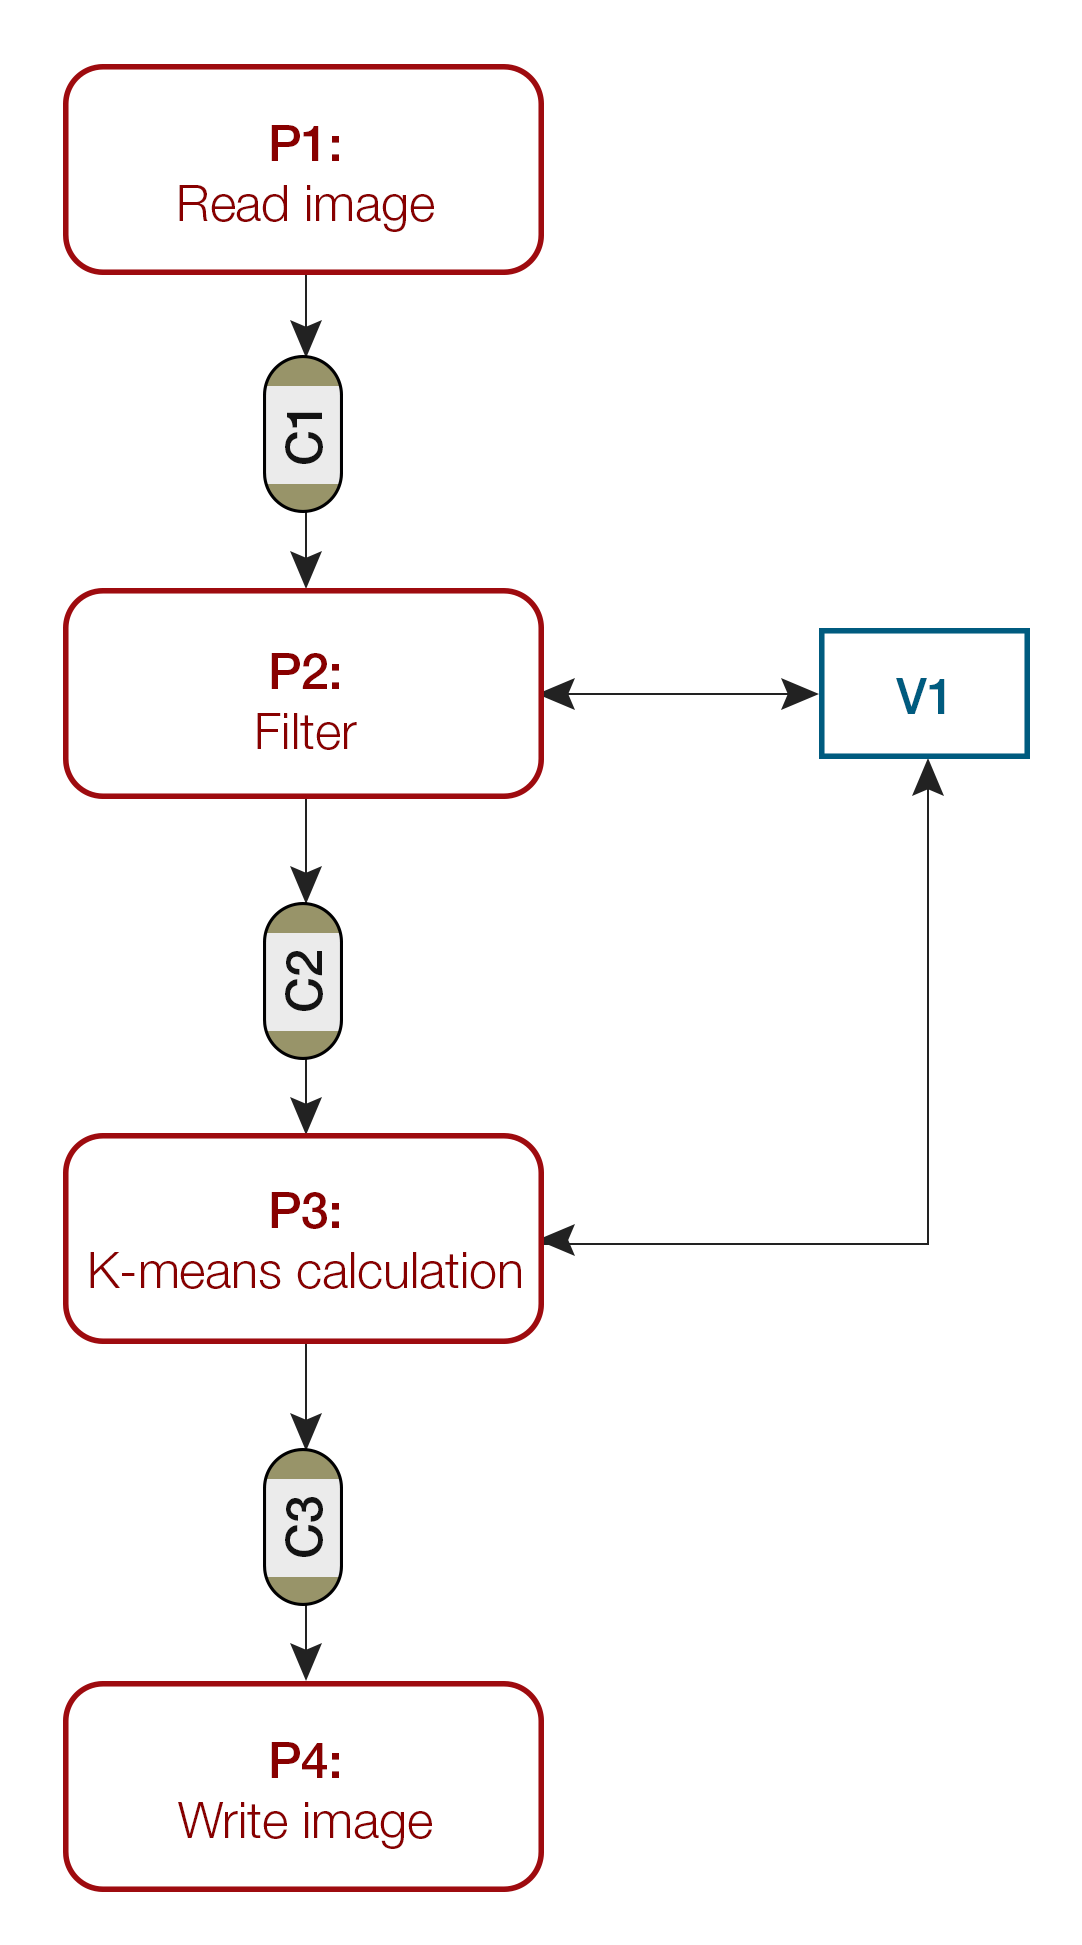
\includegraphics[width = 180 pt]{SpecificationModel}
\caption{Specification model}
\label{fig:SpecificationModel}
\end{figure}

This model serves as a basis for developing the application in terms of its behavior and performing the system synthesis.